	\begin{tabular}{ | c   p{18cm} |}
		\hline
		\cellcolor{black}\rotcell{\large\textbf{\textcolor{white}{Spezielle Relativitätstheorie}}}  &
		\setlength{\extrarowheight}{10pt}	
		
		\begin{tabular}{L{5cm} L{6.5cm} L{5.3cm}}
			&&\\[-20pt]
			\rowcolor[rgb]{1,1,1}
			\textbf{Vierervektor} \qquad\qquad $x^\mu$ Kontravarianter Vierervektor& 
			$x^\mu = 
			\left[ \begin{array}{c} ct\\
			\vec{x}\end{array}\right]	
			= 
			\left[ \begin{array}{c}
			x^0\\
			x^1\\
			x^2\\
			x^3\\
			\end{array}\right]	
			$&
			$	x_\mu = \left[ \begin{array}{c}
			ct\\
			\vec{x}
			\end{array}\right]	
			= \left[ \begin{array}{c}
			x_0\\
			x_1\\
			x_2\\
			x_3\\
			\end{array}\right]
			=x^\mu$\\[5pt]
			
	\rowcolor[rgb]{0.91,0.91,0.91}
	\textbf{Metrischer Tensor}\qquad\qquad $x_\mu$ Kovarianter Vierervektor& 
	$x_\mu = g_{\mu v}x^v$&
	
	$g_{\mu v}=\left[ \begin{array}{cccc} 
	1&0&0&0\\
	0&1&0&0\\
	0&0&1&0\\
	0&0&0&1\\
	\end{array}\right]$ \\
	
		
		
	\rowcolor[rgb]{1,1,1}
	\textbf{Gallileitransformation}& 
	$x^{'\mu} = M_{G}^{\mu v}x_v
	$&
	$M_{G}^{\mu v}=\left[ \begin{array}{cccc} 
	1&0&0&0\\
	-\beta^1&1&0&0\\
	-\beta^2&0&1&0\\
	-\beta^3&0&0&1\\
	\end{array}\right]$\\[5pt]	
		
		
	\rowcolor[rgb]{0.91,0.91,0.91}
	\textbf{Grundlagen Einstein RT}& 
	$\displaystyle \gamma=\frac{1}{\sqrt{1-\beta^2}} \quad \text{und} $\qquad $\displaystyle \beta = \frac{v}{c}$&  \\
	
	Zeitdilitation& $\Delta t = \gamma \Delta t'$ 	& \\[5pt]
	
	Längenkontraktion &$\displaystyle l = \frac{l'}{\gamma}$ & \multirow{-3}{*}{\centering 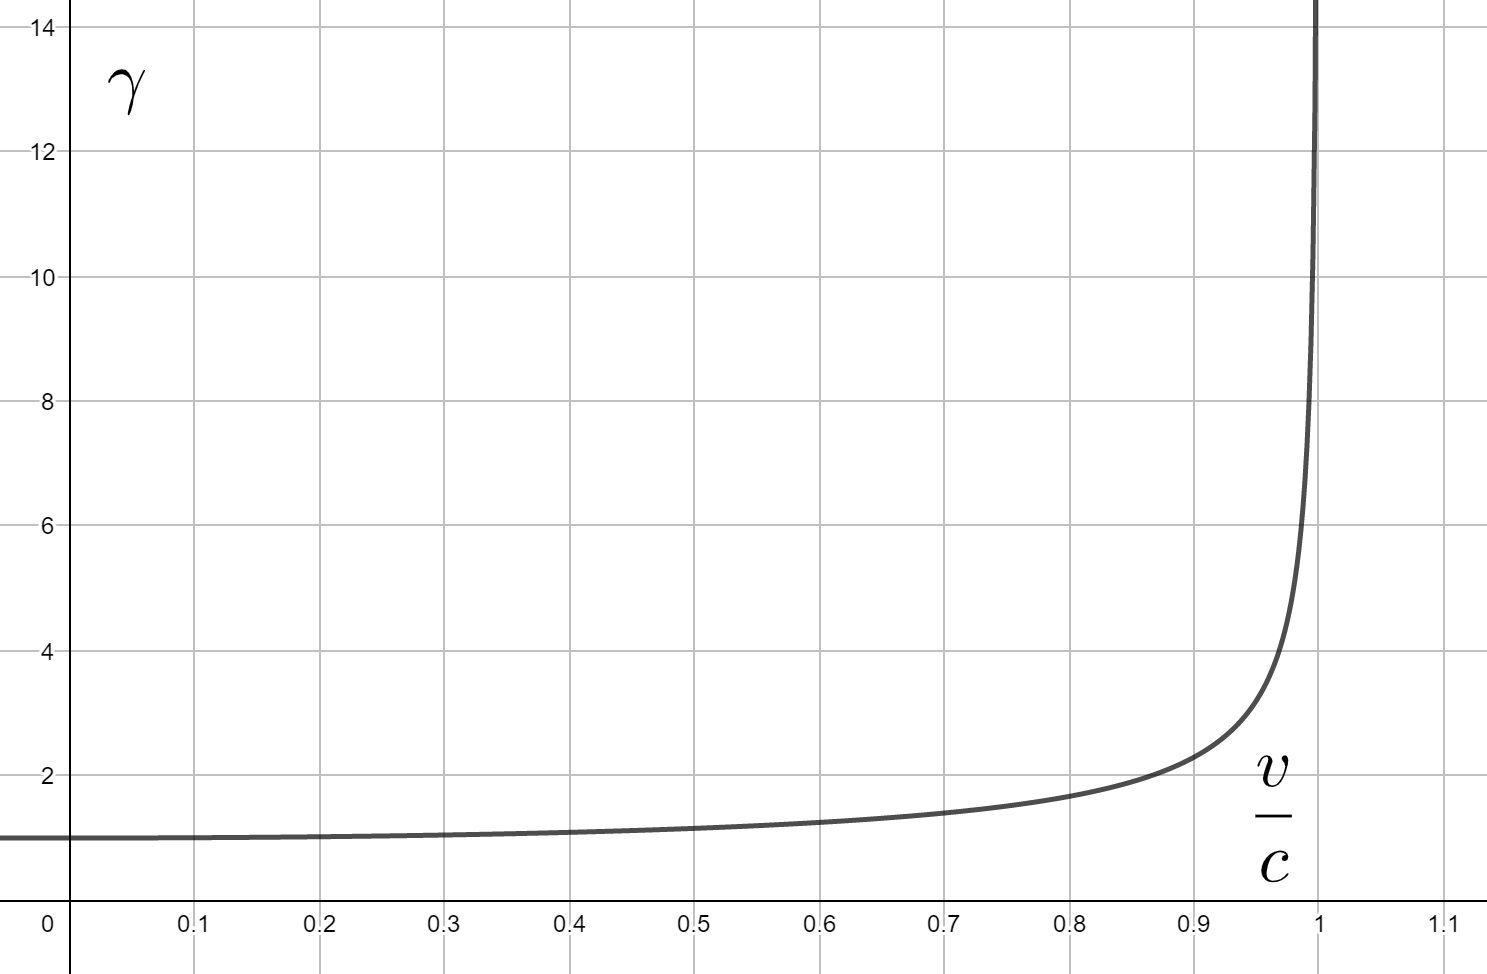
\includegraphics[width=5.5cm]{gamma.png}}\\[50pt]
	
	\rowcolor[rgb]{1,1,1}
	\textbf{Lorentz-Transformation}&
		$\left[ \begin{array}{c}
			t'\\
			x'\\
			y'\\
			z'\\
		\end{array}\right]
		=
		\left[\begin{array}{c}
			\gamma\left( t-\frac{v}{c^2}z\right)\\
			x\\
			y\\
			\gamma(z-vt)
		\end{array}\right]$&
		$\left[\begin{array}{c}
			t\\
			x\\
			y\\
			z\\
		\end{array}\right]
		=
		\left[\begin{array}{c}
				\gamma\left(t'+\frac{v}{c^2}z'\right)\\
				x\\
				y\\
				\gamma(z'+vt')
		\end{array}\right]$\\
	
	
		($\mathcal{K} \xrightarrow{v_z} \mathcal{K}'$: für $\vec{v} = v \vec{e_z}$
		eine Bewegung des Systems $\mathcal{K}'$ in $z$-Richtung)& $\displaystyle x'^\mu = \Lambda_\mu^\nu x^\nu$&
		
		$\Lambda_\mu^\nu = 
		\left[\begin{array}{cccc}
			\gamma & 0 & 0 & -\beta\gamma \\
			0 & 1 & 0 & 0\\
			0 & 0 & 1 & 0\\
			-\beta\gamma & 0 & 0 & \gamma\\
		\end{array}\right] $\\
	
	
	
		\rowcolor[rgb]{0.91,0.91,0.91}
		\textbf{Metrischer Tensor }& $\displaystyle x_\mu = g_{\mu\nu}x^\nu$ & 
		$\left[\begin{array}{cccc}
			1 & 0 & 0 & 0\\
			0 & -1 & 0 & 0\\
			0 & 0 & -1 & 0\\
			0 & 0 & 0 & -1\\
		\end{array}\right] $ \\
		
		
		\end{tabular}\\
\hline
\end{tabular}	

	
\begin{tabular}{ | c   p{18cm} |}
	\hline
	\cellcolor{black}\rotcell{\large\textbf{\textcolor{white}{Spezielle Relativitätstheorie}}}  &
	\setlength{\extrarowheight}{10pt}	
	
	\begin{tabular}{L{5cm} L{6.5cm} L{5.3cm}}
		\textbf{Raumzeit-Intervall }&$\Delta s^2 >0$ Zeitartig, $\Delta s^2 <0$ Raumartig  &\\
		\multicolumn{3}{c}{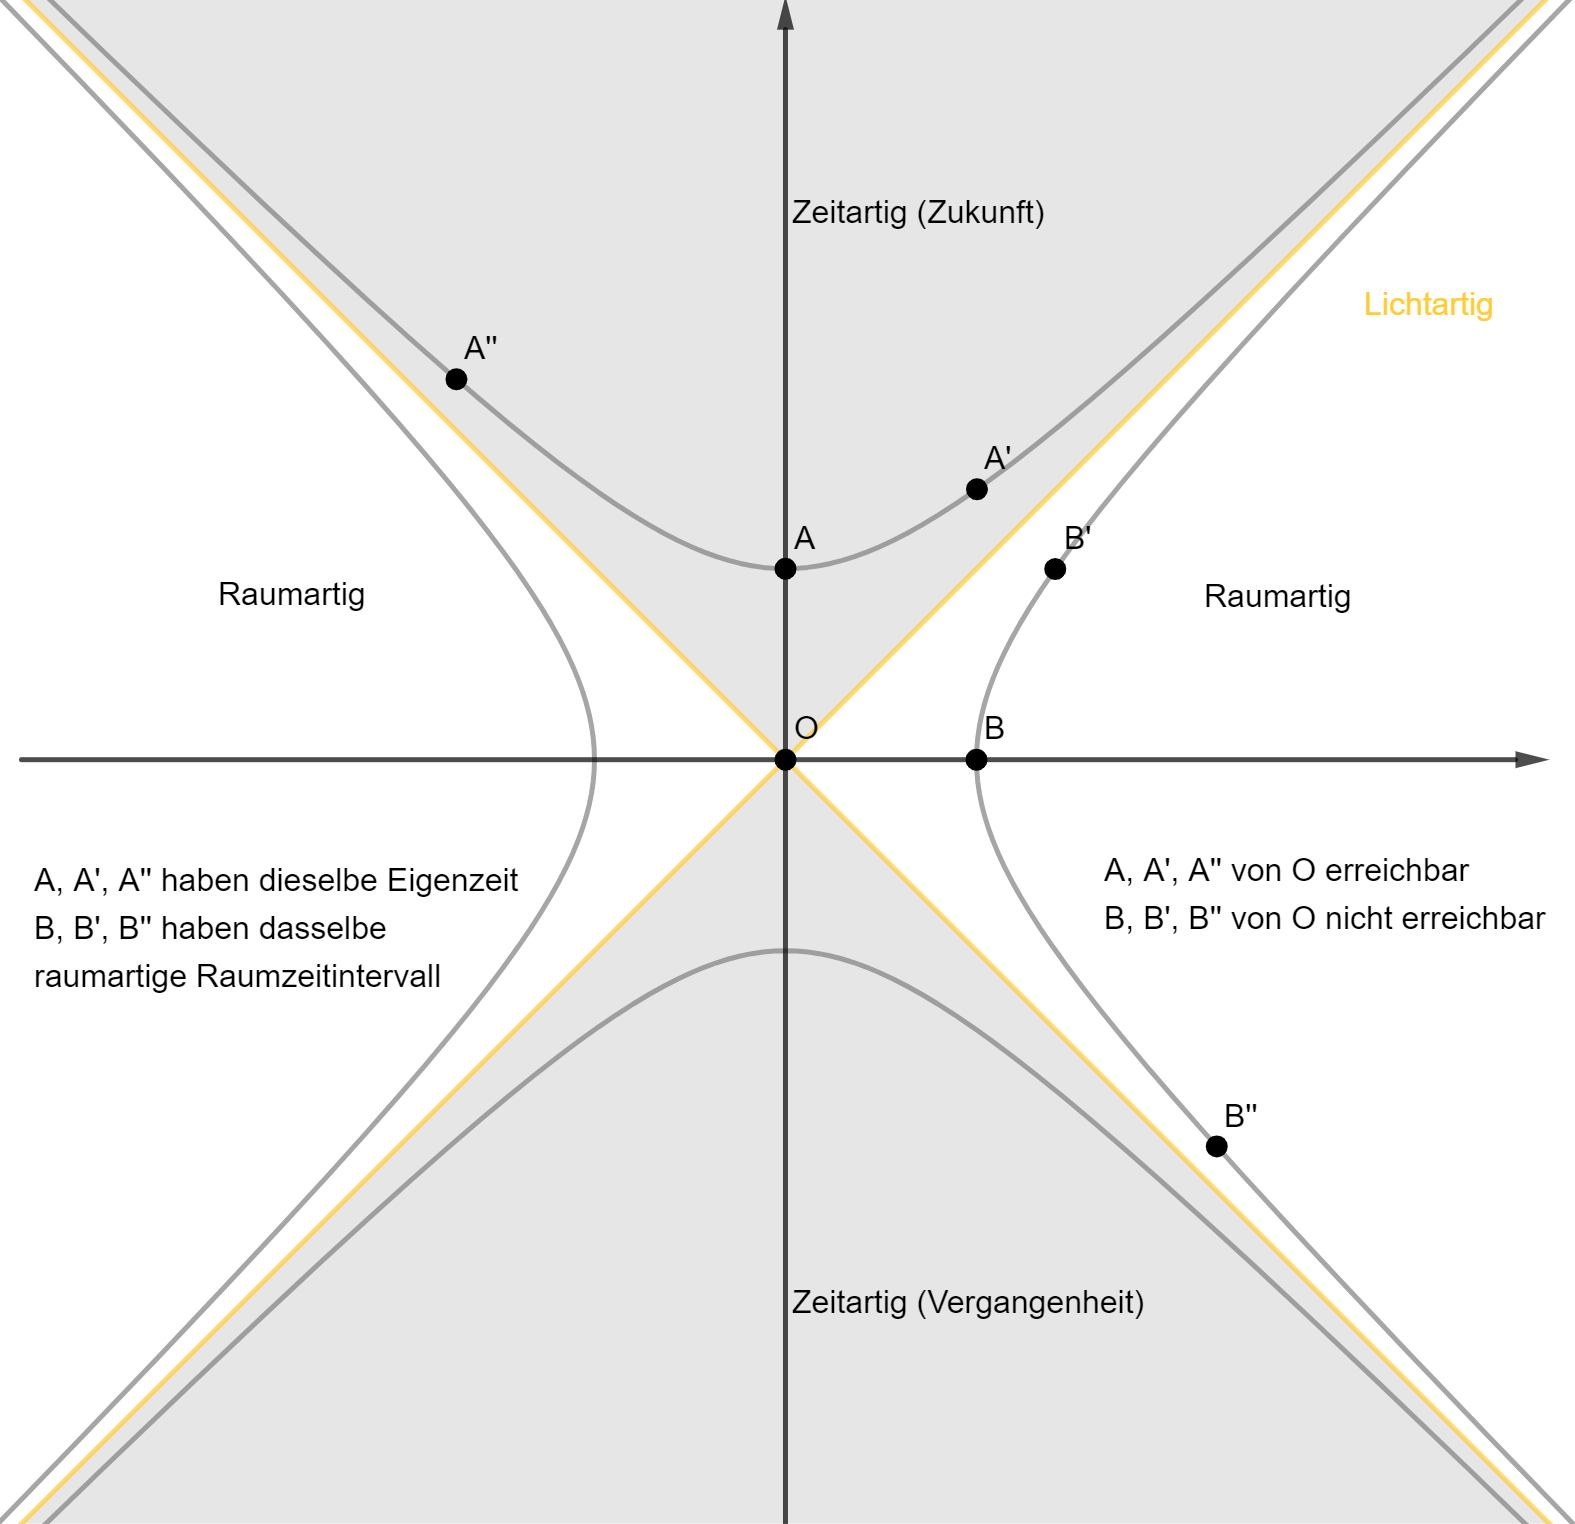
\includegraphics[width=12cm]{Minkowski.png}}\\
		 \multicolumn{3}{c}{ $\Delta s^2 = (c\Delta t)^2 -\Delta \vec{r}^2 = (c\Delta t)^2 - \Delta x^2 - \Delta y^2- \Delta z^2= \Delta x^\mu \Delta x_\mu$} \\
		
		
		\rowcolor[rgb]{0.91,0.91,0.91}
		\textbf{Geschwindigkeitsaddition}& $\displaystyle u' = \frac{u-v}{1-\frac{uv}{c^2}} \qquad\text{und}\qquad u = \frac{u'+v}{1+\frac{u'v}{c^2}}$ & $u'$ Geschwindigkeit in $\displaystyle \mathcal{K}'$, wobei $\displaystyle \mathcal{K}\xrightarrow{v}\mathcal{K}'$\\[10pt]
		

		\rowcolor[rgb]{1,1,1}
		\textbf{Ruheenergie}&$\displaystyle E_0 = mc^2$&\\

		\rowcolor[rgb]{0.91,0.91,0.91}
		\textbf{Vierergeschwindigkeit/-impuls}&$u^\mu =
			\left[\begin{array}{c}
			c\gamma\\
			c\gamma\vec{\beta}
		\end{array}\right]$ &
		$p^\mu = 
		\left[\begin{array}{c}
		mc\\
		m\vec{v}
		\end{array}\right]
		=
		\left[\begin{array}{c}
		E/c\\
		\vec{p}
		\end{array}\right]$\\
		
		&$\displaystyle E = m\gamma c^2 \qquad \text{und}$& $\displaystyle \vec{p} = m\vec{v}\gamma$\\
		
		\rowcolor[rgb]{1,1,1}
		\textbf{Betragsquadrat des Viererimpulses}&$\displaystyle p^2 = p^\mu p_\mu = \frac{E^2}{c^2}-\vec{p}^2 = m^2c^2$&\\


		\rowcolor[rgb]{0.91,0.91,0.91}
		\textbf{Kraft}& $\displaystyle m\gamma \vec{a} = \vec{F}-\frac{1}{c^2}(\vec{F}\cdot \vec{v})\vec{v}$ & \\
		
		\rowcolor[rgb]{1,1,1}
		\textbf{Allgemeiner Dopplereffekt des Lichts}&$\displaystyle \cos(\vartheta) = \frac{\cos\vartheta'+\beta}{1+\beta\cos\vartheta'} $&$\displaystyle \frac{f}{f'} = \frac{1}{\gamma(1-\beta\cos\vartheta)}$\\
		\multicolumn{3}{c}{($\mathcal{K}'$ bewegt sich mit $v$ in pos $z$-Richtung rel. zu $\mathcal{K}$ mit 
			$\vartheta'$ Aussendungswinkel zur $z$-Achse)}\\
		
		\rowcolor[rgb]{0.91,0.91,0.91}
		\textbf{Longitudinaler Dopplereffekt des Lichts}&$\displaystyle \frac{f}{f'}\Bigg\vert_{\vartheta=0} = \sqrt{\frac{1+\beta}{1-\beta}}\geq 1$ & \\[5pt]
		
		\rowcolor[rgb]{1,1,1}
		\textbf{Transversaler Dopplereffekt des Lichts}&$\displaystyle \frac{f}{f'}\Bigg\vert_{\vartheta=\frac{\pi}{2}} = \sqrt{1-\beta^2} < 1$&\\

		 
		
		
		\end{tabular}\\
		\hline
	\end{tabular}